\documentclass{beamer}
\title{Git Basics}
\author{David Kouka}
\date{\today}

\usepackage{graphicx}   % For including images
\usepackage{listings}   % For code listings

\lstset{
    basicstyle=\ttfamily\color{blue}, % Change color and font
    keywordstyle=\color{red},
    commentstyle=\color{green},
    stringstyle=\color{orange},
    columns=flexible,
    keepspaces=true,
    showstringspaces=false,
}

\begin{document}

\frame{\titlepage}  % Title slide

\section{Table of Contents}

\begin{frame}
\frame{Table of Contents}
\tableofcontents
\end{frame}

\section{Version control}

\begin{frame}{Why using version control}
    \begin{itemize}
        \item<1-> Tracking changes \lstinline{git diff} Register
        \item<2-> Backup and recovery \lstinline{git checkout} Time machine
        \item<3-> Collaborative work (authors, conflicts, PR)
        \item<4-> Accountability \lstinline{git blame}
        \item<5-> "Documentation" via commit messages \lstinline{git log}
        \item<6-> Safe experiments \lstinline{git branch} *boum*
        \item<7-> Easy release management (tags, banches, CI/CD, ...)
    \end{itemize}
\end{frame}

\section{Git commands}

\begin{frame}{Hosting}
    \only<1-> Git hosting platforms
    \begin{itemize}
        \item<2-> Bitbucket 
        \item<3-> Gitea
        \item<4-> Github
        \item<5-> Gitlab
    \end{itemize}
\end{frame}

\subsection{Cloning}
\begin{frame}{git clone}
    \only<1-> Copy repository from server \pause
    \begin{center}
        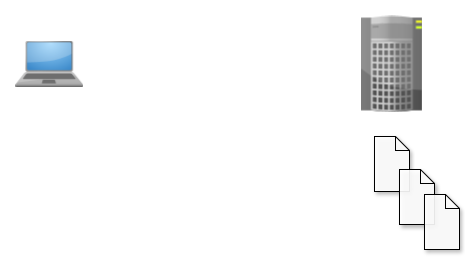
\includegraphics[width=0.5\linewidth]{img/git_clone_1.png}
    \end{center}
\end{frame}

\begin{frame}{git clone}
    Copy repository from server 
    \begin{center}
        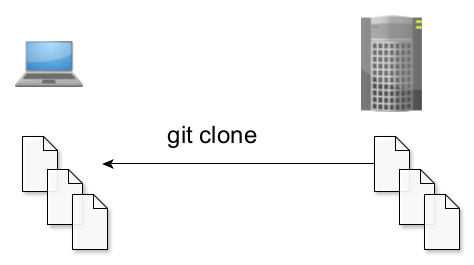
\includegraphics[width=0.5\linewidth]{img/git_clone_2.png}
    \end{center}
\end{frame}

\subsection{Stage/Commit/Push}

\begin{frame}{git add}
    \begin{center}
        
\includegraphics[width=0.5\linewidth]{img/add.png}
    \end{center}
\end{frame}


\begin{frame}{git commit}
    \begin{center}
        
\includegraphics[width=0.5\linewidth]{img/commit.png}
    \end{center}
\end{frame}

\begin{frame}{git push}
    \begin{center}
        
\includegraphics[width=0.5\linewidth]{img/push.png}
    \end{center}
\end{frame}

\subsection{Branch}

Kage bushin no jutsu
Each shadow is mastering a technique

\subsection{Merge}

Shadows goes back to the original: benefits all experiences

\subsection{Conflicts}

Conflicts: 2 ways of doing same thing (ingredients of recipe)

\end{document}

